\chapter{Validaci\'on y Resultados}
\label{chap:resultados}

%\endinput

\section{Introducci\'on}
En este cap\'itulo se presentan los distintos escenarios que fueron planteados para la validaci\'on de los procesos.\\
Dado que para la metodolog\'ia de estimaci\'on de errores que proponemos, utilizamos datos reales de una misi\'on operativa argentina, hubiera sido
deseable contar con datos de alertas de colisiones reales propios de esa misi\'on, ya que esto hubiera permitido hacer una validaci\'on end-to-end de todo el prototipo. No obstante, por cuestiones de confidencialidad, no fue posible tener acceso a esa informaci\'on.\\
Frente a este panorama, se detalla a continuaci\'on la secuencia de etapas de validaci\'on que permiten evaluar, cada una de las instancias del procesamiento.\\

En primer lugar fue fundamental corroborar las propagaciones de los TLE realizadas con la librer\'ia de python {\it{sgp4-1}} \citep{sgp4python}, para ello utilizamos la versi\'on de prueba que ofrece el software STK: {\it{System Tool Kit}} de \cite{stk}\\
Para la validaci\'on de los resultados de la implementaci\'on del m\'etodo de Osweiler en la generaci\'on de matrices de covarianza, se compararon los resultados de ARxCODE para dos de los escenarios que se publican en el trabajo.\\

El m\'etodo que se propone para la estimaci\'on de la propagaci\'on de errores, es el que m\'as dificultades present\'o para ser validado. Al basarse plenamente en los datos de la misi\'on cuyos resultados de colisi\'on de alerta no pudieron ser suministrados, fue analizado en comparaci\'on con resultados estad\'isticos globales, o sobre el estudio de encuentros de otras misiones.\\

Finalmente la implementaci\'on del c\'alculo de probabilidad de colisi\'on fue evaluado a partir de la recopilaci\'on de bibliograf\'ia con datos de encuentros anteriores.\\

\section{Implentenaci\'on del modelo SGP4 en Python}

Para la propagaci\'on de las posiciones orbitales con el modelo SGP4 (Sec. \ref{subsec:sgp4model}) utilizamos la librer\'ia de python {\bf{sgp4-1}} \citep{sgp4python}.
Luego usamos el software STK para comparar nuestras propagaciones y asegurarnos la correcta utilizaci\'on y configuraci\'on de la librer\'ia sgp4-1.\\

Se listan a continuaci\'on dos tablas con las efem\'erides de la misi\'on operativa durante los primeros cuatro minutos del d\'ia 01/01/2013.
Ambas fueron generadas a partir del mismo TLE y presentan resultados que difieren en algunos metros para los peores casos. Resultado aceptable, teniendo en cuenta que las estimaciones groseras de errores para las propagaciones hechas con TLEs y SGP4 acarrean errores de kil\'ometros o decenas de kil\'ometros.\\

\underline{TLE.}
{\small
\begin{verbatim}
1 xxxxU xxxxx   13001.74853505  .00000428  00000-0  75550-4 0  9996
2 xxxxx 098.0122 011.5654 0001526 107.5603 009.0604 14.72289948 84036
\end{verbatim}}


\begin{table}[!h]
\centering
\resizebox{14cm}{!}{
\begin{tabular}{lcccccc}
Epoca & x [km] & y [km] & z [km] & vx $[km/s]$ & vy $[km/s]$ & vz $[km/s]$\\
\hline
2013-01-01 00:00&-2372.76245& -1381.01830& 6465.57494& -6.95099& -0.93631& -2.74523\\
2013-01-01 00:01& -2784.64672& -1434.31269& 6287.6158& -6.77374& -0.83955& -3.18470\\
2013-01-01 00:02& -3185.05363& -1481.69530& 6083.67196& -6.56854& -0.73932& -3.61109\\
2013-01-01 00:03& -3572.3305& -1522.96975& 5854.58154& -6.336229& -0.63602& -4.02263\\
2013-01-01 00:04& -3944.8780& -1557.96472& 5601.28702& -6.077737& -0.53007& -4.417616\\
\hline
\label{tab:arcode}
\end{tabular}
}
\caption{Resultados que genera ARxCODE utilizando la librer\'ia sgp4 de python para la propagaci\'on.}
\end{table}

\begin{table}[!h]
\centering
\resizebox{14cm}{!}{
\begin{tabular}{lcccccc}
% \hline
\'Epoca & x [km] & y [km] & z [km] & vx [km/s] & vy [km/s] & vz [km/s]\\
\hline
2013-01-01 00:00&-2372.76302&-1381.02018&6465.57433&-6.95099&-0.93631&-2.74523\\
2013-01-01 00:01&-2784.64726&-1434.31473&6287.61518&-6.77374&-0.83955&-3.18470\\
2013-01-01 00:02&-3185.05413&-1481.69750&6083.67116&-6.56854&-0.73932&-3.61109\\
2013-01-01 00:03&-3572.33097&-1522.97210&5854.58064&-6.33622&-0.63602&-4.02263\\
2013-01-01 00:04&-3944.87849&-1557.96721&5601.28604&-6.07773&-0.53008&-4.41761
\label{tab:stk}
\end{tabular}
}
\caption{Resultados del Systems Tool Kit (STK) propagando el mismo TLE que ARxCODE.}
\end{table}


%\textcolor{red}{hacer las diferencias medias para todo un dia en python y publicarlas}

\section{Estudio de errores de TLE con datos hist\'oricos}

El trabajo de Osweiler publica los resultados de las matrices de covarianza generadas, para 6 misiones y 8 ventanas de tiempo.\\
Para la validaci\'on se tomaron dos escenarios muy diferentes en cuanto a la altura del sat\'elite: LAGEOS-1 a m\'as de $5000$ km y ICESAT a $600 $ km, Tabla \ref{tab:satescenarios}.
Se presentan a continuaci\'on las tablas con los resultados comparativos, entre los valores publicados (Tablas \ref{tab:icesatOSW} y \ref{tab:lageosOSW}) y los valores obtenidos por ARxCODE (Tablas \ref{tab:icesatARX} y \ref{tab:lageosARX})para una \'unica ventana temporal.\\
Puede apreciarse, que los errores son muy grandes para el ICESAT, de baja altura, que se ve m\'as perturbado por el efecto atmosf\'erico, que no es modelable con precisión; mientras que el LAGEOS-1 presenta errores muchos \'ordenes de magnitud menor.\\

\begin{table}
 \centering
      \begin{tabular}{cccccc}
      \hline
      Nombre & ID NORAD & Altura & Ecc. & Inclinaci\'on & B* \\
      \hline
      LAGEOS-1 & 8820 & $5850$ & $0.004$ & $109.8$ & $0.0001$ \\
      ICESAT & 27642 & $600$ & $0.0002 - 0.001$ & $94$ & var\'ia \\
      \hline
      \end{tabular}
    \caption[Sat\'elites de Estudio]{Resumen de las caracter\'isticas de los sat\'elites a analizar.}
    \label{tab:satescenarios}
\end{table}

\subsection*{Tablas comparativas ICESAT}

\begin{table}[!h]
\centering
\makebox[0pt][c]{\parbox{1.0\textwidth}{%
    \begin{minipage}[t]{0.48\hsize}\centering
     \resizebox{8cm}{!}{
    \begin{tabular}{cccc}
      \hline
    Vent 1 & $R_{v}$ (km) & $R_{n}$ (km) & $R_{c}$ (km)\\
    \hline
    $R_{v}$ &  2667.377375  &    27.248658   &   -8.22221222\\
    $R_{n}$ & 27.248658  &   0.34323269 & -0.12314379\\
    $R_{c}$ & -8.22221222 & -0.12314379 & 0.07316443\\
    \hline
    \end{tabular}}
      \caption{Matriz de Covarianza de la Bibliograf\'ia \citep{osweiler} - Sat\'elite ICESAT en la ventana temporal del 1-Mar-03 al 16-Mar-03}
      \label{tab:icesatOSW}
    \end{minipage}
    \begin{minipage}[t]{0.48\hsize}\centering
    \resizebox{8cm}{!}{
      \begin{tabular}{cccc}
	\hline
      Vent 1 & $R_{v}$ (km) & $R_{n}$ (km) & $R_{c}$ (km)\\
      \hline
      $R_{v}$ &  2667.37364259 &   27.2488814  &   -8.22232626\\
      $R_{n}$ & 27.2488814  &  0.3432413 &  -0.12314867\\
      $R_{c}$ & -8.22232626 & -0.12314867 &  0.073167\\
      \hline
      \end{tabular}}
        \caption{Matriz de Covarianza que produce ARxCODE - Sat\'elite ICESAT en la ventana temporal del 1-Mar-03 al 16-Mar-03}
        \label{tab:icesatARX}
    \end{minipage}
    \hfill
}}
\end{table}

\begin{table}[!h]
\centering
 \begin{tabular}{cccc}
  \hline
 Vent 1 & Dif.$R_{v}$ (km) & Dif.$R_{n}$ (km) & Dif.$R_{c}$ (km)\\
 \hline
 Dif. $R_{v}$ & -0.00373241 & 0.0002234 & -0.00011404 \\
 Dif. $R_{n}$ &  0.0002234 &  0.000008 & -0.000004\\
 Dif. $R_{c}$ & -0.00011404  & -0.000004 &  0.000002\\
 \hline
 \end{tabular}
 \caption{Diferencias de los valores calculados por ARxCODE respecto a los valores publicados en el trabajo de Osweiler \citep{osweiler}}
 \label{tab:icesatcomp}
\end{table}


\subsection*{Tablas comparativas LAGEOS-1}


\begin{table}[!h]
\centering
\makebox[0pt][c]{\parbox{1.0\textwidth}{%
    \begin{minipage}[b]{0.48\hsize}\centering
    \resizebox{8cm}{!}{
      \begin{tabular}{cccc}
	\hline
      Vent 1 & $R_{v}$ (km) & $R_{n}$ (km) & $R_{c}$ (km)\\
      \hline
      $R_{v}$ &  0.37863904 & -0.03440871 & 0.02772177 \\
      $R_{n}$ & -0.03440871 & 0.00401173 & -0.00272334 \\
      $R_{c}$ & 0.02772177 & -0.00272334 & 0.00843443\\
      \hline
      \end{tabular}}
        \caption{Matriz de Covarianza de la Bibliograf\'ia \citep{osweiler}- Sat\'elite LAGEOS-1 en la ventana temporal del 1-Mar-03 al 16-Mar-03}
        \label{tab:lageosOSW}
    \end{minipage}
    \hfill
    \begin{minipage}[b]{0.48\hsize}\centering
     \resizebox{7.5cm}{!}{
    \begin{tabular}{cccc}
      \hline
    Vent 1 & $R_{v}$ (km) & $R_{n}$ (km) & $R_{c}$ (km)\\
    \hline
    $R_{v}$ & 0.378619 & -0.0343598 & 0.02771527 \\
    $R_{n}$ & -0.0343598 &  0.004002 & -0.0027171 \\
    $R_{c}$ & 0.02771527 & -0.0027171 &  0.0084302 \\
    \hline
    \end{tabular}}
      \caption{Matriz de Covarianza que produce ARxCODE - Sat\'elite LAGEOS-1 en la ventana temporal del 1-Mar-03 al 16-Mar-03}
      \label{tab:lageosARX}
   \end{minipage}
    \hfill
}}
\end{table}

\begin{table}[!h]
\centering
 \begin{tabular}{cccc}
  \hline
 Vent 1 & Dif.$R_{v}$ (km) & Dif.$R_{n}$ (km) & Dif.$R_{c}$ (km)\\
 \hline
 Dif. $R_{v}$ & 0.000020 &  -0.000048 &  0.000006 \\
 Dif. $R_{n}$ & -0.000048 &   0.000009 &  -0.000006 \\
 Dif. $R_{c}$ & 0.000006 &  -0.000006 &   0.000004 \\
 \hline
 \end{tabular}
 \caption{Diferencias de los valores calculados por ARxCODE respecto a los valores publicados en el trabajo de Osweiler.}
 \label{tab:lageoscomp}
\end{table}

Las diferencias que resultan en la comparaci\'on con los resultados que arroja ARxCODE, son todas menores a los metros (Tablas \ref{tab:icesatcomp} y \ref{tab:lageoscomp}).\\
En particular LAGEOS muestra errores menores que ICESAT, ya que al ser un sat\'elite a mayor altura, el efecto atmosf\'erico es menor y el modelo de propaci\'on, se adapta mejor.\\


\subsection*{Diferencias de los escenarios iterando el TLE primario en el m\'etodo de Osweiler}
Estudio hecho sobre los errores que se producen en las propagaciones de los TLE en funci\'on de la cantidad de d\'ias que se propaguen.\\
Estos resultados ofrecen mayor informaci\'on respecto a los errores que se comenten en funci\'on de la cantidad de d\'ias que se propagan los TLE.\\
Para la generaci\'on de los datos, se propagaron todos los TLE del conjunto hacia las fechas de todos los TLE con fechas m\'as actualizadas, dentro del conjunto, Fig. \ref{fig:todosOSW}. Las diferencias que resultaron se plasman en funci\'on del intervalo de propagaci\'on, en las Fig. \ref{fig:icesatTot} y Fig. \ref{fig:lageosTot} para el ICESAT y el LAGEOS respectivamente. 


\begin{figure}[!h]
\centering
  \textbf{Propagaci\'on y comparaci\'on de TLE }\par\medskip
  \fbox{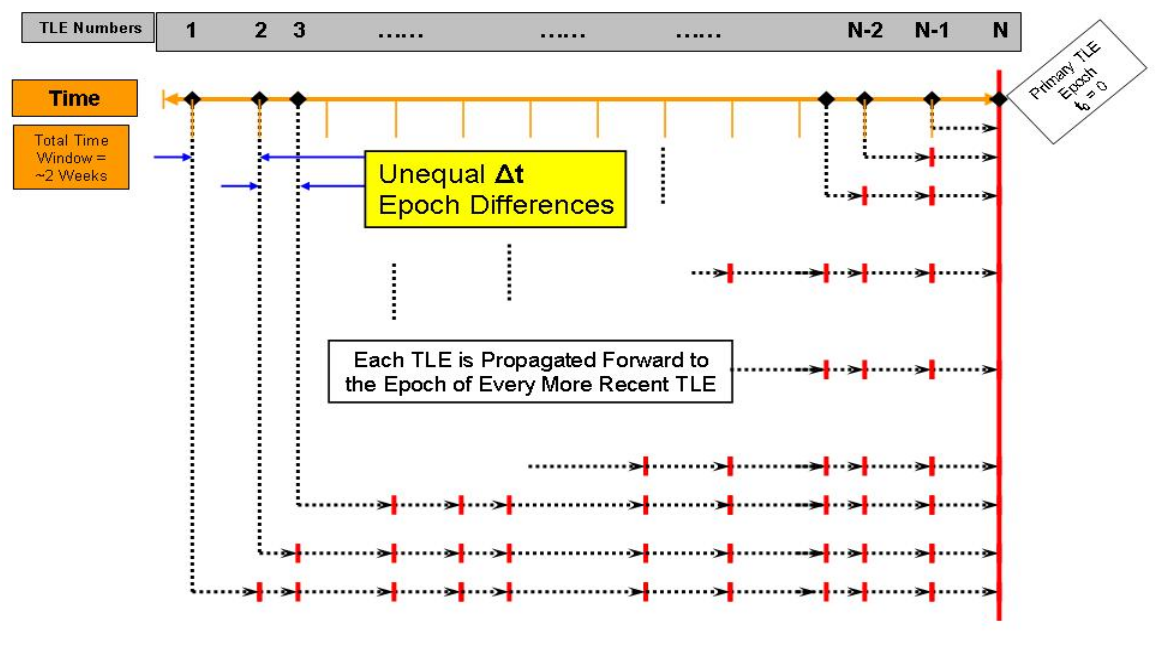
\includegraphics[width=0.8\textwidth]{imagenes/todosOSW}}
  \caption{Esquematizaci\'on del algoritmo para comparar la propagaci\'on de cada TLE del set hacia fechas futuras de los TLE del set. Extra\'ido de \cite{osweiler}}
  \label{fig:todosOSW}
\end{figure}

\begin{figure}[h!]
\centering
  \subfigure[Diferencias ICESAT - ARxCODE]{
    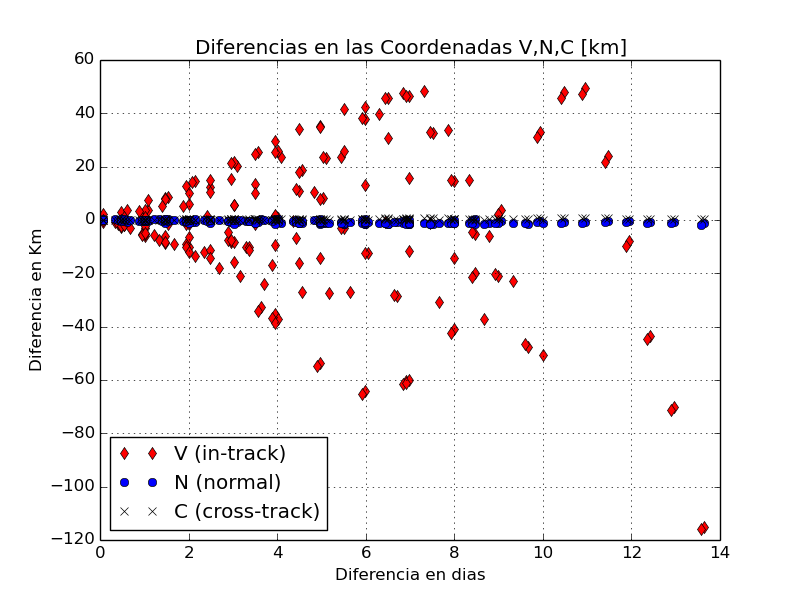
\includegraphics[width=0.48\textwidth]{imagenes/TLEdifTot27642esc52}
  }
  \subfigure[Diferencias ICESAT - Osweiler]{
    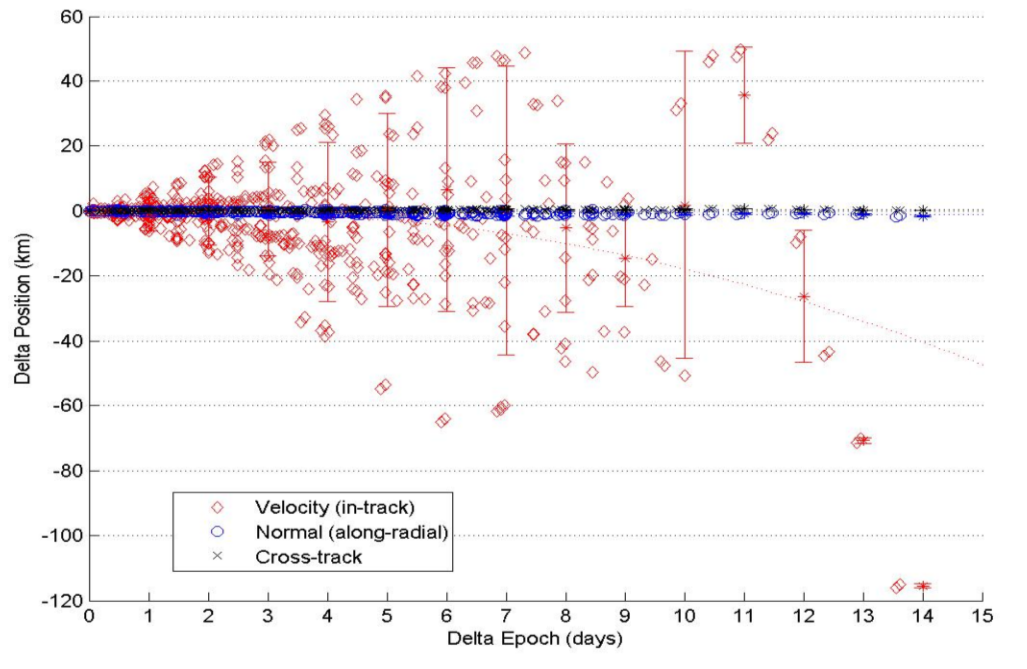
\includegraphics[width=0.48\columnwidth, keepaspectratio]{imagenes/ICESATdifTot}
  }
  \caption{Gr\'afico con Diferencias Totales del escenario ICESAT}
  \label{fig:icesatTot}
\end{figure}

\begin{figure}[h!]
\centering
  \subfigure[Diferencias LAGEOS-1 - ARxCODE]{
    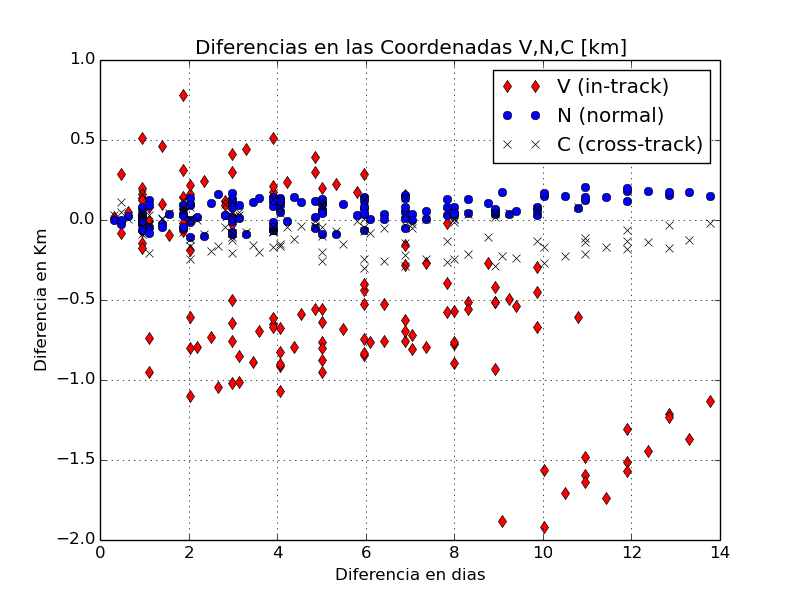
\includegraphics[width=0.48\textwidth]{imagenes/TLEdifTot8820esc11}
  }
  \subfigure[Diferencias LAGEOS-1 - Osweiler]{
    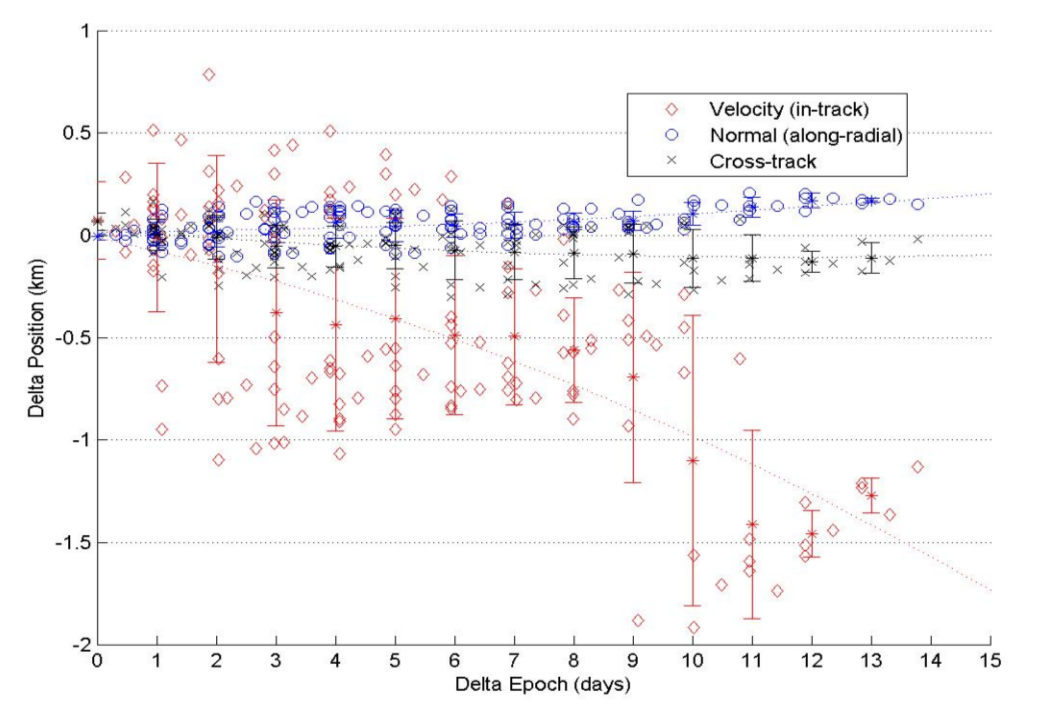
\includegraphics[width=0.48\columnwidth, keepaspectratio]{imagenes/LAGEOSdifTot}
  }
  \caption{Gr\'afico con Diferencias Totales del escenario LAGEOS-1}
  \label{fig:lageosTot}
\end{figure}

Los errores que se observan en la propagaci\'on de TLE, en funci\'on de la cantidad de d\'ias propagados, muestran comportamientos casi id\'enticos.\\
En este estudio, puede apreciarse una clara diferencia en las cotas de los errores, siendo el sat\'elite ICESAT, de menor altura el que muestra errores mayores en un rango de -120 a 60 km, mientras que el LAGEOS, contiene las diferencias entre -2 y 1 km.\\
No obstante, en ambos se distingue, que la componente asociada a la velocidad (V {\it{in-track}}) es la que mayor error acumula en propagaciones m\'as largas. Esto se debe a que el modelo es d\'ebil en cuanto a la perturbaci\'on que introduce la atm\'osfera, directamente vinculada a la velocidad de los objetos para el caso del ICESAT o en cuanto al modelo que describe la presi\'on de radiaci\'on solar en el caso del LAGEOS.\\

Se concluye a partir de esta secci\'on, que ARxCODE implementa el m\'etodo de Osweiler y la construcci\'on de las diferencias de pares correctamente. 

\section{Estudio de errores de TLE con efem\'erides precisas}
\subsection*{Sistema de referencia TOD}
La misi\'on operativa ofrece mediciones propias de sus efem\'erides.\\
En esta secci\'on se muestran los resultados de comparar las posiciones obtenidas mediante los datos p\'ublicos TLE, propagadas con SGP4, contra las efem\'erides precisas.\\ 

En primer lugar fue necesario plasmar las posiciones en el mismo sistema de referencia, ya que los productos del departamento de din\'amica orbital con los que trabajamos ofrecen las posiciones orbitales en el sistema de referencia verdadero de la fecha \ac{TOD}, mientras que los resultados de las propagaciones con el SGP4 se encuentran en el sistema \ac{TEME}. Para poder hacer comparaciones desarrollamos un m\'odulo que transforma las coordenadas y velocidades, del sistema TEME al sistema TOD (Ap\'endice. \ref{App1}).\\

Para la validaci\'on del mismo, utilizamos TLE de la misi\'on y los propagamos con el SGP4. Los resultados que obtuvimos (en el sistema TEME), los transformamos al sistema TOD con el m\'odulo de transformaci\'on desarrollado y luego lo comparamos con los productos del STK, corridos para el mismo TLE y publicados en el sistema TOD que STK ofrece. Las comparaciones se hicieron para propagaciones con paso de 1 minuto a lo largo de todo el dia 01 de Enero de 2013. Los resultados mostraron diferencias menores a los mil\'imetros, de manera que el algoritmo puede usarse sin que incorpore errores significativos.\\

\begin{table}
\centering
\begin{tabular}{l|c}
  \hline
  Coordenada  X &  0.0003168 [m]\\
  Coordenada Y &  0.0006370 [m]\\
  Coordenada Z &  0.0005133 [m]\\
  \hline
\end{tabular}
\caption{Valores Medios en la comparaci\'on de los resultados de la transformaci\'on de TEME a TOD de ARxCODE, con los resultados que ofrece el software STK. Propagaciones para todo el d\'ia 1 de Enero de 2013, con paso 1 minuto.}
\end{table}

\subsection*{Estad\'istica de Errores}
Con la certeza de que los datos eran compatibles y pod\'ian ser comparados (ambos se referencian en el sistema TOD), se inici\'o el procesamiento de comparaci\'on de las posiciones de las efem\'erides precisas de la misi\'on y las propagaciones de los TLE, para la estimaci\'on de los errores de la propagaci\'on, Sec. \ref{subsec:errorProp}.

En un pre-procesamiento sobre un periodo amplio de la misi\'on, constatamos que fuera de los intervalos de maniobras por {\it{commissioning}}\footnote{Puesta en \'orbita nominal} o maniobras de rutina, los TLE presentan un error que es {\it{acotado}}, {\it{estable}} y/o modelable. \\

Las comparaciones de las propagaciones de los TLE mostraron significativas aleatoriedades y amplias diferencias en el estudio realizado con los datos correspondientes al a\~no 2012, no obstante los resultados del estudio con datos del a\~no 2013 mostraron la tendencia y estabilidad esperada, ver Fig. \ref{fig:sacd2013}, con errores m\'aximos del orden de las decenas de kil\'ometros.


\begin{figure}[!h]
\centering
  \textbf{Tendencia Anual 01/01/2013 - 30/08/2013}\par\medskip
  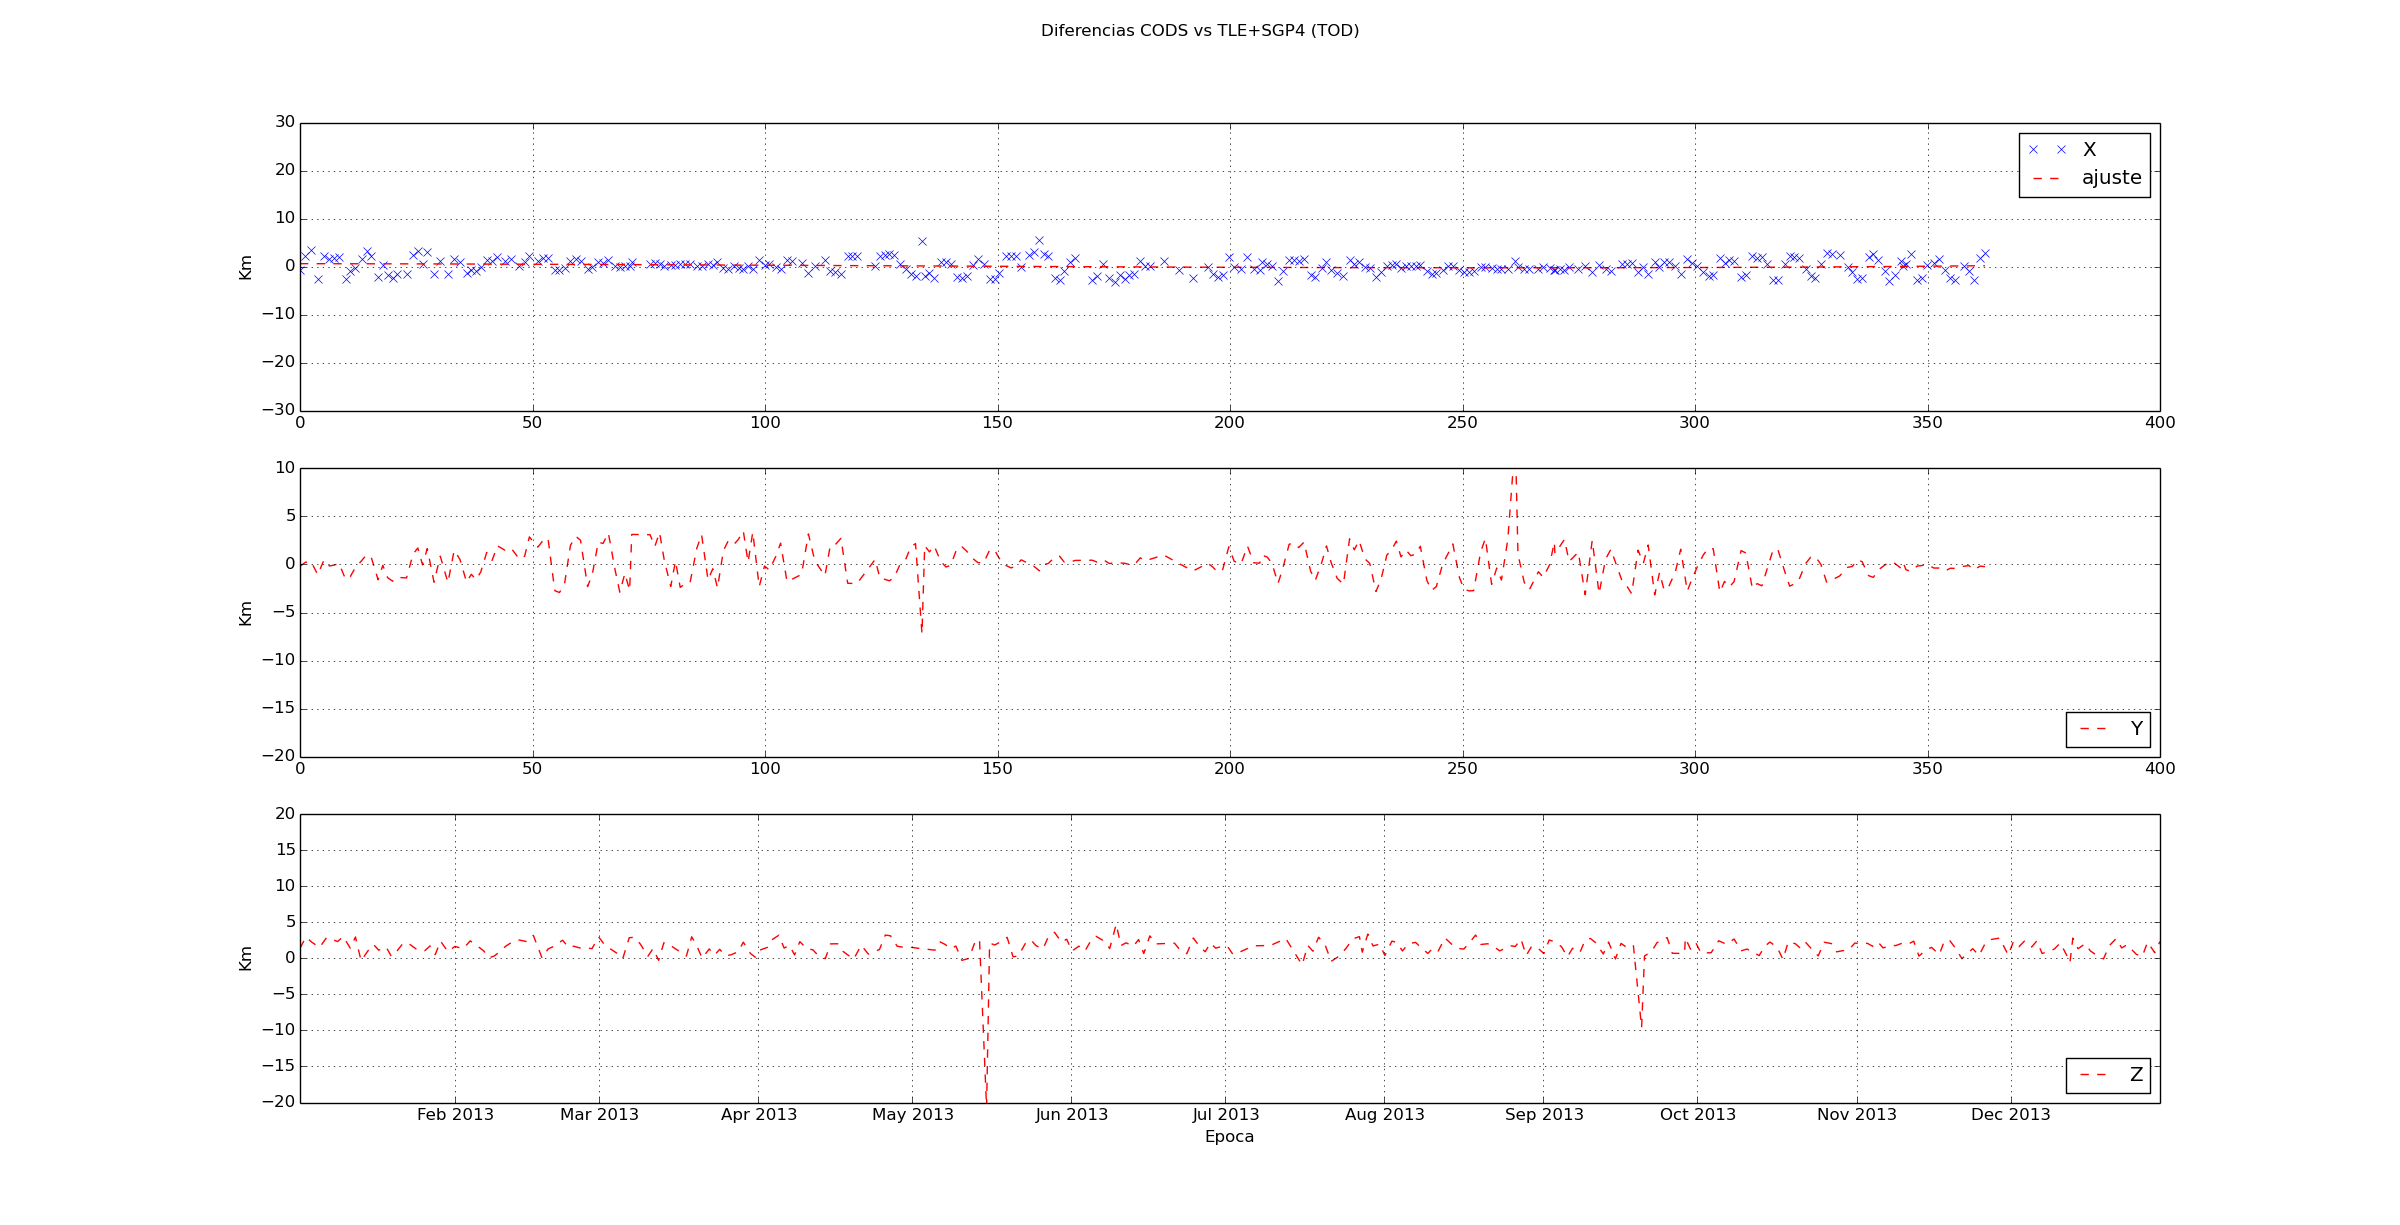
\includegraphics[width=0.9\textwidth]{imagenes/SACD2013todEjesajustados}
  \caption{Tendencia anual de las diferencias contra los datos de din\'amica orbital en coordenadas cartesianas del Sistema TOD}
  \label{fig:sacd2013}
\end{figure}

\subsection*{Generaci\'on de la tabla de propagaci\'on de errores}

Como se explic\'o en la Sec. \ref{subsec:errorProp}, para estimar los errores en la propagaci\'on se propone un m\'etodo que utiliza una tabla, Tab. \ref{tab:resultatabla}, generada a partir de la estad\'istica que resulta de comparar las propagaciones de los TLE de la misi\'on operativa, con las efem\'erides precisas. Las comparaciones se hacen en el periodo de Enero a Junio del a\~no 2013, en intervalos de 1 a 6 d\'ias, con paso 1 segundo.\\
Los resultados que se encuentran, no es posible validarlos directamente. No obstante, son comparables a los que proponen \cite{flohrer2008assessment}, en la {\it{lookup table}} generada considerando todos los objetos del cat\'alogo al 01 de Enero de 2008, ver Fig. \ref{fig:flohrer}. Los valores de las desviaciones est\'andar que resultan del m\'etodo propuesto son menores casi en un orden de magnitud a las tablas gen\'ericas que publican \cite{flohrer2008assessment}, esto es de esperar, ya que los estudios de la publicaci\'on son m\'as abarcativos y gen\'ericos.\\

\begin{table}[!h]
\centering

\begin{tabular}{|l|c|c|c|}
\hline \hline
\rowcolor{yellow!35}
&$\sigma^{2}_R [km]$ &$\sigma^{2}_T [km]$ &$\sigma^{2}_N [km]$\\
\hline \hline
< 1 d\'ia & 0.05287535953&0.5110606907&0.09802202353\\
\hline
1 d\'ia & 0.03846388969&0.4517572281&0.09807457894\\
\hline
2 d\'ias & 0.02760890529&0.4086434248&0.09904162392\\
\hline
3 d\'ias & 0.01963580775&0.3765098311&0.09022336881\\
\hline
4 d\'ias & 0.01469071678&0.3577884914&0.1182060362\\
\hline
5 d\'ias & 0.01332578794&0.3557767231&0.1264764812\\
\hline
6 d\'ias & 0.01524829841&0.365815954&0.1607439516\\
\hline
\end{tabular}
\caption[Tabla con los valores medios para la propagaci\'on de errores.]{Resultados finales de los valores medios de las varianzas calculadas para la propagaci\'on de errores en funci\'on de los d\'ias de propagaci\'on. Autor\'ia propia.}
\label{tab:resultatabla}
\end{table}

\begin{figure}[!h]
  \centering
  \fbox{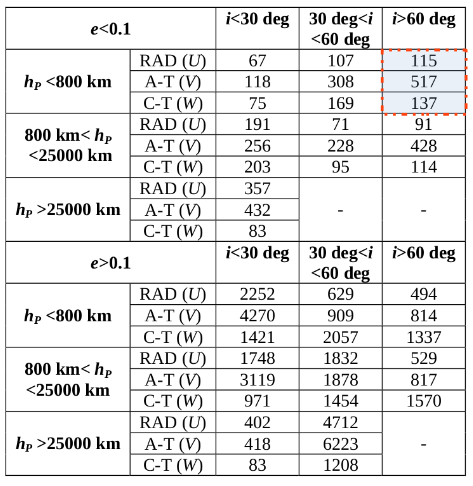
\includegraphics[width=0.6\textwidth]{imagenes/flohrertabla}}
  \caption{{\it{Look-up table}} [metros] de los resultados promediados del an\'alisis del cat\'ologo completo al 01 de Enero de 2008, de los errores en las coordenadas UVW, clasificados por excentricidad, inclinaci\'on y altura. Se resaltan en celeste las celdas correspondientes a la configuraci\'on de la misi\'on operativa que se utiliz\'o en este trabajo. Extra\'ido de \cite{flohrer2008assessment}}
  \label{fig:flohrer}
\end{figure}

% \begin{itemize}
%  \item Klinkrad Tabla para 14 misiones.
%  \item Paper del research gate
%  \item Peterson?!
% \end{itemize}
% 
% FINALIZAR CON COMPARACI\'ON TLE vs TLE. 

\section{C\'alculo de la Probabilidad de Colisi\'on}

El c\'alculo de la PoC, implementa la expresi\'on presentada por  \cite{leichen}.


\subsection*{Comparaci\'on de los resultados con la resoluci\'on de la integral}
Con el objeto de verificar los c\'alculos que se realizan en el m\'odulo, se toman como datos iniciales, los valores publicados por el propio autor Lei-Chen, y se calcula la PoC, tanto para la expresi\'on anal\'itica como la integral. Para esta \'ultima se utiliza la biblioteca {\it{scipy.integrate}}  de python.

De las expresiones para el c\'alculo de la PoC (Eq. \ref{eq:pocintegral} y Eq. \ref{eq:pocexpress}), se desprende que ser\'an necesarios los datos: ($\mu_{x}, \mu_{y}$), ($\sigma_{x}, \sigma_{y}$), $r_{a}$.\\
Se tomaron los datos que utiliza Lei-Chen en el ejemplo para el caso de las \'orbitas circulares y se calcul\'o la PoC a partir de la expresi\'on expl\'icita y realizando la integral.\\

\begin{minipage}[t]{0.28\textwidth}
{\bf{Valores iniciales.}}\\

\begin{tabular}{|lc|}
\hline
 Dato & valor \\
\hline
$\mu_{x}$ & 0.031731 [km]\\
$\mu_{y}$ & 0.697294 [km]\\
$\sigma_{x}$ & 0.0430576\\
$\sigma_{y}$ & 0.2941297\\
$r_{a}$ & 0.01 [km]\\
\hline
\end{tabular}
\end{minipage}
\begin{minipage}[t]{0.7\textwidth}
\begin{mdframed}[
        linecolor=red,linewidth=2pt,% 
        frametitlerule=true,% 
        apptotikzsetting={\tikzset{mdfframetitlebackground/.append style={%
            shade,left color=white, right color=blue!20}}}, 
        frametitlerulecolor=blue,
        frametitlerulewidth=1pt, innertopmargin=\topskip,
        frametitle={Probabilidad de Colisi\'on},
        outerlinewidth=1.25pt
    ]
\large

\begin{tabular}{|l|l|l|}
  \hline
 Te\'orico & Expresi\'on & Valor de la Integral\\
 \hline
 1.8079750e-04 & 1.8079124e-04 & 1.8071110e-04\\
 \hline
\end{tabular}
\captionof{table}{Resultados Comparativos del c\'alculo de la PoC.}
\label{tab:poccomp}
\end{mdframed}
\end{minipage}

\vspace{0.5cm}
Como se observa en el recuadro de las probabilidades de colisi\'on (Tabla \ref{tab:poccomp}); las f\'ormulas implementadas coinciden con el valor de la bibliograf\'ia hasta el cuarto d\'igito significativo de la expresi\'on.\\

En este punto se confirma que, una vez que se obtiene: $\mu_{x}$, $\mu_{x}$, $\sigma_{x}$, $\sigma_{y}$ y el radio de colisi\'on $r_{a}$, ya puede calcularse la PoC. 
Ahora resta verificar, paso a paso c\'omo llegar de los inputs de ARxCODE, a estos par\'ametros que se introducen en de las ecuaciones. \\

\subsection*{C\'alculos previos}

Una vez determinadas la posici\'on relativa de los objetos en el sistema RSW o RTN en el TCA, la proyecci\'on al plano para \'orbitas circulares, no representa mayores problemas, como se detall\'o en la Sec. \ref{subsec:pocsimp}.\\

Pero es importante verificar, que a partir de las posiciones inerciales de los objetos en el TCA, las transformaciones de la distancia relativa de los mismos al sistema RSW, coincide.\\
Para ello, vamos a utilizar las posiciones de los objetos del ejemplo de la bibliograf\'ia (Tabla \ref{tab:vectejemplo}) y transformarlas con el m\'odulo de transformaci\'on {\it{sisRic}} del paquete {\it{SistReferencia.SistdeCoordenadas}} para corroborar los resultados.
\\

\begin{table}[!h]
\centering
\begin{tabular}{l|c|c|c|c|c|c}
\hline
Objeto & x [km] & y [km] &z[km] &vx [km] &vy [km] &vz [km]\\
\hline
Obj1 & 1457.273246 &1589.568484&6814.189959&7.001731&2.439512&0.926209\\
\hline
Obj2 & 1457.532155&1588.932671&6814.316188&3.578705&6.172896&2.200215\\
\hline
\end{tabular}
\caption{Vectores de Posiciones Inerciales al momento TCA. Extra\'idos del ejemplo de la bibliograf\'ia \citep{leichen}}
\label{tab:vectejemplo}
\end{table}

\begin{table}[!h]
\large
 \centering
\begin{tabular}{|l|c|c|c|}
\hline
Resultados seg\'un & R [km] & S [km] & W[km] \\
\hline
Lei Chen & 0.031731& 0.436476&0.543785\\
\hline
ARxCODE & 0.031797& 0.462295 &0.522013
\\
\hline
\end{tabular}
\caption{Resultados comparativos de la transformaci\'on entre sistemas de referencia utilizando el m\'odulo {\it{sisRic}} de autor\'ia propia y los datos de la bibliograf\'ia \citep{leichen}.}
\label{tab:rswcomp}
\end{table}

Estos resultados que se publican en la tabla \ref{tab:rswcomp}, se logran en una transformaci\'on en la que se considere al Obj2 como origen de la referencia. Los mismos muestran una coincidencia del orden de las decenas de metros, aceptable para estas estimaciones.\\
No obstante, contando s\'olo con la informaci\'on de los vectores de posici\'on al momento del m\'aximo acercamiento, no es posible verificar el m\'etodo de Osweiler de la construcci\'on de la matriz de covarianza para este ejemplo de la bibliograf\'ia.\\

\subsection*{Validaci\'on end-to-end}
Hasta este punto, se han ido validando cada uno de los procesos por separado.\\
Resta hacer pruebas desde el origen, es decir a partir de identificar los objetos y el TCA, correr los procesamientos de ARxCODE y obtener los resultados de la PoC.\\
A tal fin, fue necesario conseguir registros que contuvieran la informaci\'on completa de una situaci\'on de encuentro.\\
Esto no fue posible en su totalidad. Por un lado tuvimos acceso a mails de alerta p\'ublicos en internet, y por otro a CDM tambi\'en p\'ublicos\footnote{https://cwe.ccsds.org/moims/docs/Forms/AllItems.aspx?RootFolder=\%2Fmoims\%2Fdocs\%2FMOIMS-NAV\%2FDraft\%20Documents\%2FConjunction\%20Data\%20Message\%20\%28CDM\%29}, pero ninguno de esos datos se corresponden con la misi\'on operativa, cuyas efem\'erides precisas analizamos y utilizamos en la construcci\'on del modelo estad\'istico de propagaci\'on de errores.\\
As\'i mismo, ni los mails encontrados ni los CDM descargados, contienen informaci\'on de la PoC asociada al encuentro. \\

\subsubsection*{Validaci\'on con correos electr\'onicos de alerta p\'ublicos}

El proceso de validaci\'on utilizando los correos electr\'onicos obtenidos en la web, consiste de extraer de los correos los identificadores de norad de ambos objetos y el TCA asociado al encuentro. A partir de all\'i se calcula la m\'inima distancia total, o sea el m\'odulo de la misma, y  en componentes en el sistema RTN y finalmente la PoC.\\
Dado que el TCA que se publica en los correos no tiene informaci\'on de los segundos, se realiza una primera estimaci\'on, y luego se profundiza en an\'alisis de la situaci\'on.\\

Formato de los correos electr\'onicos:\\
\begin{center}
\fbox{\parbox[b]{0.8\linewidth}{
The United States Joint Space Operations Center (JSpOC) has identified a\\
predicted conjunction between DELFI C3 (SCC\# 32789) and SCC\# 23657.\\

Primary Object: DELFI C3 (SCC\# 32789)\\
Secondary Object: SCC\# 23657\\
Time of Closest Approach: 15 JUL 2012 21:21 UTC \\

Overall miss distance: 760 meters\\
Radial (dU) miss distance: -186 meters\\
In-Track (dV) miss distance: -389 meters\\
Cross-track (dW) miss distance: -626 meters\\

Primary Radial Error (U): 38 meters\\
Primary In-track Error (V): 1388 meters\\
Primary Cross-track Error (W): 11 meters\\

Secondary Radial Error (U): 8 meters\\
Secondary In-track Error (V): 338 meters\\
Secondary Cross-track Error (W): 2 meters\\
}}
\end{center}

{\bf{Nota:}} Los los correos electr\'onicos no informan los segundos del TCA. Fue necesario primero hacer una primera estimaci\'on m\'as precisa del TCA del encuentro y luego volver a procesar incorporando los segundos. 

Listado de Mails analizados:\\

\begin{figure}[!h]
  \centering
  \fbox{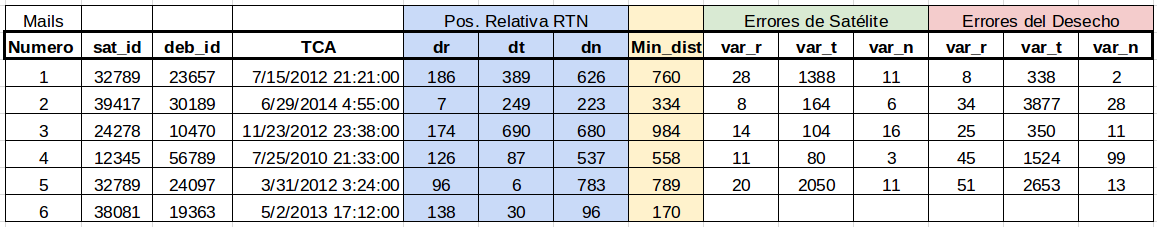
\includegraphics[width=\textwidth]{imagenes/tablamails}}
  \caption{Contenido de los correos electr\'onicos utilizados para comparar los resultados.}
  \label{fig:tablamails}
\end{figure}

Valores de ARxCODE:\\
\begin{table}[!h]
\resizebox{16cm}{!}{
\begin{tabular}{|l|r|r|r|r|r|r|}
 \hline \hline
 \# & TCA arx & $\Delta R_{arx}$ [m] & $\Delta T_{arx}$ [m] & $\Delta N_{arx}$ [m] & Min Dist. arx [m] & PoC arx\\
 \hline \hline
 1 & 2012-07-15 21:21:51 & 147.106 & 2749.095 &  2287.11 & 3579 & 6.426171e-22 \\
 \hline
 2 & 2014-06-29 04:55:59 & 81.349 & 3921.163 & 2002.826 & 4403 & 0.0 \\
 \hline
 3 & 2012-11-23 23:38:42 & 0300.62 & 1668.766 & 841.432 & 1892 & 0.0 \\
 \hline
 4 & 2013-03-31 03:25:45 & 68.072008 & 1.318496 & 426.131856 & 431.536667 & 0.0 \\
 \hline
 5 & xxxxxx & xxxxxx & xxxxxx & xxxxxx & xxxxxx & xxxxxx \\
 \hline
\end{tabular} }
\caption{Resultados que se obtienen con ARxCODE a partir de la informaci\'on de los correos electr\'onicos, propagando cada 1 segundo}
\end{table}


\begin{table}[!h]
\resizebox{16cm}{!}{
\begin{tabular}{|l|r|r|r|r|r|r|}
 \hline \hline
 \# & TCA arx & $\Delta R_{arx}$ [m] & $\Delta T_{arx}$ [m] & $\Delta N_{arx}$ [m] & Min Dist. arx [m] & PoC arx\\
 \hline \hline
 1 & 2012-07-15 21:21:51.3 & 0.142965 & 0.512276 &  0.254972 & 0.58981 & 4e-06 \\
 \hline
 2 & 2014-06-29 04:55:59.1 & 0.0824 & 3.253859 & 2.745704 & 4.25831 & 0.0 \\
 \hline
 3 & 2012-11-23 23:38:42.1 & 0.258083 & 0.936411 & 1.595317 & 1.86775 & 1.7e-05 \\
 \hline
 4 & 2013-03-31 03:25:45.1 & 68.075882 & 0.194278 & 426.131566 & 431.535022 & 0.0 \\
 \hline
 5 & 2013-05-02 17:12:02.9 & 20.173626 & 504.135854 & 146.837803 & 525.47243 & 0.0\\
 \hline
\end{tabular} }
\caption{Resultados que se obtienen con ARxCODE incorporando a la informaci\'on de los correos electr\'onicos, el valor de los segundos en el TCA y propagando cada 100.000 microsegundos}
\end{table}

Las matrices de covarianza no mejoran. Ver tabla \ref{fig:tablaMAmails}

 \begin{figure}[!h]
  \centering
  \fbox{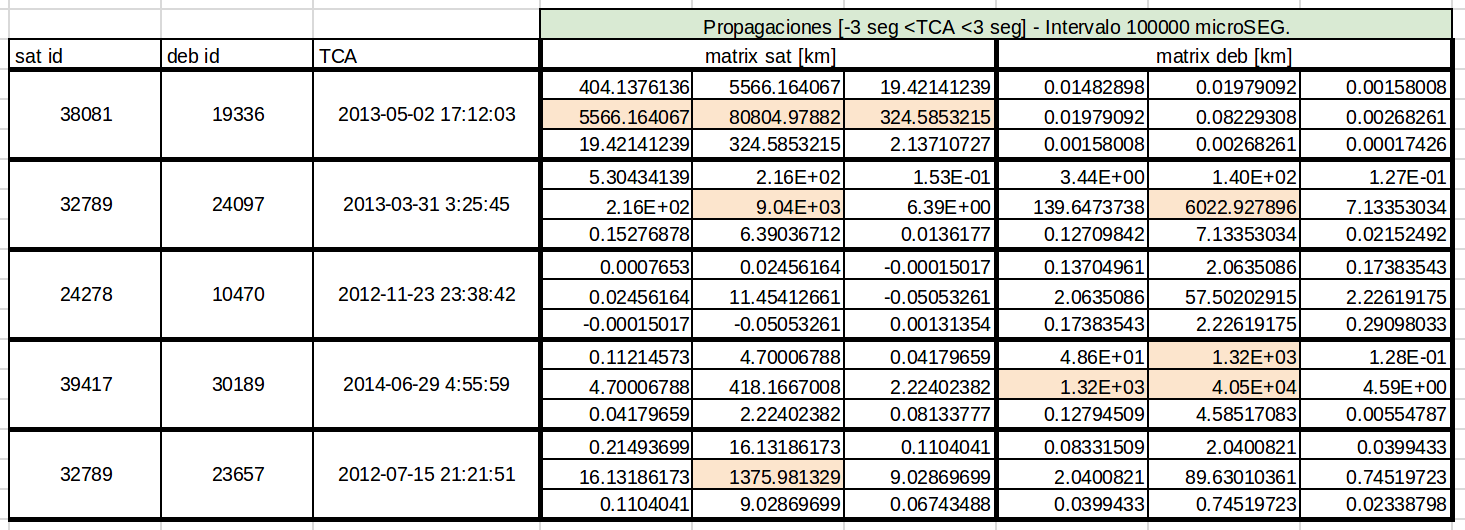
\includegraphics[width=\textwidth]{imagenes/tablaMAmails}}
  \caption{Tabla con las matrices de covarianza para la misi\'on y el desecho.}
  \label{fig:tablaMAmails}
\end{figure}

\subsubsection*{Validaci\'on con CDM p\'ublicos}
 
 \begin{figure}[!h]
  \centering
  \fbox{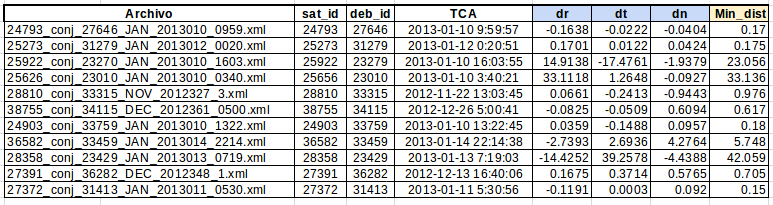
\includegraphics[width=\textwidth]{imagenes/tablaCDM}}
  \caption{Contenido de los CDM utilizados para comparar los resultados.}
  \label{fig:tablamails}
\end{figure}
 
 \begin{table}[!h]
 \resizebox{16cm}{!}{
\begin{tabular}{|l|r|r|r|r|r|r|}
 \hline \hline
 \# & TCA arx & $\Delta R_{arx}$ [km] & $\Delta T_{arx}$ [km] & $\Delta N_{arx}$ [km] & Min Dist. arx [km] & PoC arx\\
 \hline \hline
 1 & 2013-01-10 09:59:57 &0.295626&1.358542&1.321294&1.918033& 1.1e-05 / 1.1e-05\\
 \hline
 2 & 2013-01-12 00:20:51 &0.405629&4.127385&1.632732&4.457091&0.0 / 0.0\\
 \hline 
 3 & 2013-01-10 13:22:45 & 0.382972 & 1.173174  & 1.316177 & 1.804252 & 8e-06\\
 \hline 
 4 & 2013-01-11 05:30:56 & 0.01038& 1.276203& 0.648991&1.431779&0.0\\
 \hline 
 5 & 2012-11-22 13:03:45.000823 & 0.027395 & 4.661372 & 0.332569 & 4.673301 & 1.4e-05/1.4e-05 \\
 \hline
 6 & 2012-12-26 05:00:41 & 0.183897& 4.661359&0.02668&4.665061& 1e-06 / 1e-06\\
 \hline
 \end{tabular} }
 \caption{Resultados que se obtienen con ARxCODE a partir de la informaci\'on de los CDM, propagando cada 1 segundo}
 \end{table}
 
\begin{table}[!h]
 \resizebox{16cm}{!}{
\begin{tabular}{|l|r|r|r|r|r|r|}
 \hline \hline
 \# & TCA arx & $\Delta R_{arx}$ [km] & $\Delta T_{arx}$ [km] & $\Delta N_{arx}$ [km] & Min Dist. arx [km] & PoC arx\\
 \hline \hline
 1 &2013-01-10 09:59:57  &0.295626&1.358542& 1.321294&1.918033&1.4e-05 \\
 \hline
 2 & 2013-01-12 00:20:51.3 &0.401158&0.140306&0.218037&0.477654&6.1e-05\\
 \hline
 3 & 2013-01-10 13:22:45.2 & 0.382381 &0.288759& 0.043842&0.481165&9e-06\\
 \hline
 4 &2013-01-11 05:30:55.9&0.016754 &0.215364 &0.573953&0.613257&0.0\\
 \hline
 5 & 2012-11-22 13:03:44.700823 & 0.023908 & 0.436662& 0.758981 & 0.875955 & 2e-05 \\
 \hline
 6 & 2012-12-26 05:00:40.7 & 0.183162& 0.1859&00.417861&0.492661& 1.24e-04\\
 \hline
 \end{tabular} }
 \caption{Resultados que se obtienen con ARxCODE incorporando la informaci\'on de los mails, el valor de los segundos en el TCA y propagando cada 100.000 microsegundos}
 \end{table}

\newpage
\section{An\'alisis} 
 A partir de estos resultados, se desprenden los siguientes an\'alisis:\\
 
 \begin{itemize}
  \item Las funcionalidades para la conexi\'on con NORAD para la descarga de TLE, y las propagaciones que se realizan de los mismos, funcionan correctamente.\\
  \item El m\'etodo de Osweiler para la generaci\'on de la matriz de covarianza, resulta con diferencias del orden de los cent\'imetros respecto de los valores publicados. Resultado m\'as que aceptable dado que las \'orbitas m\'as precisas que se consideran en este trabajo tienen errores del orden de 20 metros.\\
  \item El estudio de los errores en funci\'on de la cantidad de d\'ias que se propaguen los TLE coincide con los resultados publicados por Osweiler y respeta los valores esperados, de acuerdo a los efectos perturbativos y las caracter\'isticas de las \'orbitas de los sat\'elites analizados.\\
  \item Las tendencias en los errores que se obtienen al comparar las propagaciones de los TLE con las efem\'erides precisas a lo largo del a\~no 2013, mostraron un comportamiento estable y acotado, salvo outliers, como se esperaba. Con cotas superiores de decenas de kil\'ometros.\\
  \item La metodolog\'ia utilizada para estimar errores en la propagaci\'on, mostr\'o resultados comparables y a\'un mejores que los propuestos por \cite{flohrer2008assessment}.
  \item Las transformaciones al sistema de referencia RTN tienen diferencias del orden de las decenas de metros con las publicadas en el ejemplo de Lei-Chen.\\
  \item No se cuenta con datos para poder validar las proyecciones de la posici\'on relativa y la matriz de covarianza al plano de encuentro.\\
  \item Se utilizaron correos electr\'onicos de alertas y CDM que son p\'ublicos en internet para validar las diferencias que se obtienen entre las distancias m\'inimas que estos datos contienen y las distancias m\'inimas calculadas por ARxCODE. Las diferencias resultan muy notorias en la primera instanca en la que se itera con paso un segundo, pero mejoran significativamente reduciendo el paso de integraci\'on a las d\'ecimas de segundos. No obstante, desconociendo el origen de los correos electr\'onicos y los CDM, no todo puede atribuirse al procesamiento de ARxCODE.\\
  \item Utilizando los mismos correos electr\'onicos y CDM se calculan las probabilidades de colisi\'on con ARxCODE, aunque el resultado no puede compararse, ya que ni los correos electr\'onicos, ni los CDM que se obtuvieron contienen esa informaci\'on. Los valores asociados a los correos electr\'onicos (que son los que cuentan con mayor diferencia en las m\'inimas distancias) dan siempre nulos en las propagaciones con pasos del segundo, y algunos resultados mejoran al achicar el paso. En cambio, en los resultados asociados a los CDM se encuentran valores aceptables en ambos casos, aunque mejores para las iteraciones menores al segundo.\\
 \end{itemize}
